\documentclass{article}\usepackage[]{graphicx}\usepackage[]{color}
% maxwidth is the original width if it is less than linewidth
% otherwise use linewidth (to make sure the graphics do not exceed the margin)
\makeatletter
\def\maxwidth{ %
  \ifdim\Gin@nat@width>\linewidth
    \linewidth
  \else
    \Gin@nat@width
  \fi
}
\makeatother

\definecolor{fgcolor}{rgb}{0.345, 0.345, 0.345}
\newcommand{\hlnum}[1]{\textcolor[rgb]{0.686,0.059,0.569}{#1}}%
\newcommand{\hlstr}[1]{\textcolor[rgb]{0.192,0.494,0.8}{#1}}%
\newcommand{\hlcom}[1]{\textcolor[rgb]{0.678,0.584,0.686}{\textit{#1}}}%
\newcommand{\hlopt}[1]{\textcolor[rgb]{0,0,0}{#1}}%
\newcommand{\hlstd}[1]{\textcolor[rgb]{0.345,0.345,0.345}{#1}}%
\newcommand{\hlkwa}[1]{\textcolor[rgb]{0.161,0.373,0.58}{\textbf{#1}}}%
\newcommand{\hlkwb}[1]{\textcolor[rgb]{0.69,0.353,0.396}{#1}}%
\newcommand{\hlkwc}[1]{\textcolor[rgb]{0.333,0.667,0.333}{#1}}%
\newcommand{\hlkwd}[1]{\textcolor[rgb]{0.737,0.353,0.396}{\textbf{#1}}}%
\let\hlipl\hlkwb

\usepackage{framed}
\makeatletter
\newenvironment{kframe}{%
 \def\at@end@of@kframe{}%
 \ifinner\ifhmode%
  \def\at@end@of@kframe{\end{minipage}}%
  \begin{minipage}{\columnwidth}%
 \fi\fi%
 \def\FrameCommand##1{\hskip\@totalleftmargin \hskip-\fboxsep
 \colorbox{shadecolor}{##1}\hskip-\fboxsep
     % There is no \\@totalrightmargin, so:
     \hskip-\linewidth \hskip-\@totalleftmargin \hskip\columnwidth}%
 \MakeFramed {\advance\hsize-\width
   \@totalleftmargin\z@ \linewidth\hsize
   \@setminipage}}%
 {\par\unskip\endMakeFramed%
 \at@end@of@kframe}
\makeatother

\definecolor{shadecolor}{rgb}{.97, .97, .97}
\definecolor{messagecolor}{rgb}{0, 0, 0}
\definecolor{warningcolor}{rgb}{1, 0, 1}
\definecolor{errorcolor}{rgb}{1, 0, 0}
\newenvironment{knitrout}{}{} % an empty environment to be redefined in TeX

\usepackage{alltt}
\PassOptionsToPackage{unicode}{hyperref}
\PassOptionsToPackage{naturalnames}{hyperref}
\usepackage{fullpage}
\usepackage[T2A]{fontenc}
\usepackage[utf8]{inputenc}
\usepackage[russian]{babel}
\usepackage{mathrsfs}
\usepackage{amsfonts}
\usepackage{amsmath }
\IfFileExists{upquote.sty}{\usepackage{upquote}}{}
\begin{document}
\title{Отчет по домашнему заданию}
\pretitle{\vspace{\droptitle}\centering\huge}
\posttitle{\par}
\author{Фахртдинов Т. А.}


\maketitle

Вторая задача. Оценка параметров.
Вариант 4.

1) Промоделировать выборки объемом 100 и 300 имеющие сложно пуассоновское с внутренним геометрическим распределением. Ввиду того, что параметры не были уточнены, я взял произвольные значения параметров распределения, $\lambda = 3$, $p$ = 0.5:
\begin{knitrout}
\definecolor{shadecolor}{rgb}{0.969, 0.969, 0.969}\color{fgcolor}\begin{kframe}
\begin{alltt}
\hlstd{generate_pois.geom} \hlkwb{<-} \hlkwa{function}\hlstd{(}\hlkwc{size}\hlstd{)\{}
  \hlstd{samp} \hlkwb{<-} \hlkwd{character}\hlstd{()}
  \hlkwa{for} \hlstd{(j} \hlkwa{in} \hlnum{1}\hlopt{:}\hlstd{size) \{}
    \hlstd{x} \hlkwb{<-} \hlkwd{rpois}\hlstd{(}\hlnum{1}\hlstd{,} \hlnum{3}\hlstd{)}
    \hlstd{y} \hlkwb{<-} \hlkwd{rgeom}\hlstd{(x,} \hlnum{0.5}\hlstd{)}
    \hlstd{samp} \hlkwb{<-} \hlkwd{c}\hlstd{(samp,} \hlkwd{sum}\hlstd{(y))}
  \hlstd{\}}
  \hlstd{samp} \hlkwb{<-} \hlkwd{as.numeric}\hlstd{(samp)}
  \hlkwd{return}\hlstd{(samp)}
\hlstd{\}}

\hlstd{first} \hlkwb{<-} \hlkwd{generate_pois.geom}\hlstd{(}\hlnum{100}\hlstd{)}
\hlstd{second} \hlkwb{<-} \hlkwd{generate_pois.geom}\hlstd{(}\hlnum{300}\hlstd{)}

\hlstd{n1} \hlkwb{<-} \hlkwd{length}\hlstd{(first)}
\hlstd{n2} \hlkwb{<-} \hlkwd{length}\hlstd{(second)}
\end{alltt}
\end{kframe}
\end{knitrout}
2) Теперь оценим параметры используя метод моментов.
Известно, что производящие функции моментов распределения Пуассона и распределения Бернулли соответственно имеют вид:
$$f(s) = e^{-\lambda + s\lambda}$$
$$g(s) = \frac{p}{1 - qs}$$
тогда получаем производящую функцию сложного распределения:
$$h(s) = f(g(s)) = e^{-\lambda + \lambda  \frac{p}{1 - qs}}$$
$$\alpha_1 = h'(1)$$
$$\eta_2 = h''(1) + h'(1) - (h'(1))^2$$
$h'(1) = \frac{q\lambda}{p}$ \; $h''(1) = \frac{q^2(\lambda^2 + 2\lambda)}{p^2}$
\newline
\newline
$\alpha_1 = \frac{q\lambda}{p}$ \; $\eta_2 = \frac{qp\lambda + 2q^2\lambda}{p^2}$
\newline
Из чего мы получаем оценки:
$$\bar p = \frac{2}{m_2 + \bar x}$$
$$\bar \lambda = \frac{2 \bar x^2}{m_2 - \bar x}$$

\begin{knitrout}
\definecolor{shadecolor}{rgb}{0.969, 0.969, 0.969}\color{fgcolor}\begin{kframe}
\begin{alltt}
\hlstd{estimate_p} \hlkwb{<-} \hlkwa{function}\hlstd{(}\hlkwc{samp}\hlstd{)\{}
  \hlkwd{return}\hlstd{(}\hlnum{2} \hlopt{/} \hlstd{(}\hlkwd{var}\hlstd{(samp)} \hlopt{+} \hlkwd{mean}\hlstd{(samp)))}
\hlstd{\}}

\hlstd{estimate_lmbd} \hlkwb{<-} \hlkwa{function}\hlstd{(}\hlkwc{samp}\hlstd{)\{}
  \hlkwd{return}\hlstd{(} \hlnum{2} \hlopt{*} \hlkwd{mean}\hlstd{(samp)}\hlopt{^}\hlnum{2} \hlopt{/} \hlstd{(}\hlkwd{var}\hlstd{(samp)} \hlopt{-} \hlkwd{mean}\hlstd{(samp)))}
\hlstd{\}}
\end{alltt}
\end{kframe}
\end{knitrout}


Для первой:
\begin{knitrout}
\definecolor{shadecolor}{rgb}{0.969, 0.969, 0.969}\color{fgcolor}\begin{kframe}
\begin{alltt}
\hlstd{lmbd_f} \hlkwb{<-} \hlkwd{estimate_lmbd}\hlstd{(first)}
\hlstd{p_f} \hlkwb{<-} \hlkwd{estimate_p}\hlstd{(first)}
\hlstd{lmbd_f}
\end{alltt}
\begin{verbatim}
## [1] 2.927628
\end{verbatim}
\begin{alltt}
\hlstd{p_f}
\end{alltt}
\begin{verbatim}
## [1] 0.1697094
\end{verbatim}
\end{kframe}
\end{knitrout}
Для второй:
\begin{knitrout}
\definecolor{shadecolor}{rgb}{0.969, 0.969, 0.969}\color{fgcolor}\begin{kframe}
\begin{alltt}
\hlstd{lmbd_s} \hlkwb{<-} \hlkwd{estimate_lmbd}\hlstd{(second)}
\hlstd{p_s} \hlkwb{<-} \hlkwd{estimate_p}\hlstd{(second)}
\hlstd{lmbd_s}
\end{alltt}
\begin{verbatim}
## [1] 2.747303
\end{verbatim}
\begin{alltt}
\hlstd{p_s}
\end{alltt}
\begin{verbatim}
## [1] 0.1383145
\end{verbatim}
\end{kframe}
\end{knitrout}

Построим доверительные интервалы.

Начнем с параметра p:
\begin{knitrout}
\definecolor{shadecolor}{rgb}{0.969, 0.969, 0.969}\color{fgcolor}\begin{kframe}
\begin{alltt}
\hlstd{DH_p} \hlkwb{<-} \hlkwa{function}\hlstd{(}\hlkwc{samp}\hlstd{)\{}
  \hlstd{m} \hlkwb{<-} \hlkwd{mean}\hlstd{(samp)}
  \hlstd{a2} \hlkwb{<-} \hlkwd{mean}\hlstd{(samp}\hlopt{^}\hlnum{2}\hlstd{)}
  \hlstd{a3} \hlkwb{<-} \hlkwd{mean}\hlstd{(samp}\hlopt{^}\hlnum{3}\hlstd{)}
  \hlstd{a4} \hlkwb{<-} \hlkwd{mean}\hlstd{(samp}\hlopt{^}\hlnum{4}\hlstd{)}
  \hlstd{m2} \hlkwb{<-} \hlstd{a2} \hlopt{-} \hlstd{m}\hlopt{^}\hlnum{2}
  \hlstd{m3} \hlkwb{<-} \hlstd{a3} \hlopt{-} \hlnum{3} \hlopt{*} \hlstd{a2} \hlopt{*} \hlstd{m} \hlopt{+} \hlnum{2} \hlopt{*} \hlstd{m}\hlopt{^}\hlnum{3}
  \hlstd{m4} \hlkwb{<-} \hlstd{a4} \hlopt{-} \hlnum{4} \hlopt{*} \hlstd{a2} \hlopt{*} \hlstd{m} \hlopt{+} \hlnum{6} \hlopt{*} \hlstd{a2} \hlopt{*} \hlstd{m}\hlopt{^}\hlnum{2} \hlopt{-} \hlnum{3} \hlopt{*} \hlstd{m}\hlopt{^}\hlnum{4}
  \hlstd{n} \hlkwb{<-} \hlkwd{length}\hlstd{(samp)}
  \hlstd{dh} \hlkwb{<-} \hlstd{(m2} \hlopt{/} \hlstd{n} \hlopt{+} \hlnum{2} \hlopt{*} \hlstd{(n} \hlopt{-} \hlnum{1}\hlstd{)} \hlopt{*} \hlstd{m3} \hlopt{/} \hlstd{n}\hlopt{^}\hlnum{2} \hlopt{+} \hlstd{(m4} \hlopt{-} \hlstd{m2}\hlopt{^}\hlnum{2}\hlstd{)} \hlopt{/} \hlstd{n)} \hlopt{*} \hlnum{4} \hlopt{/} \hlstd{((m2} \hlopt{+} \hlstd{m)}\hlopt{^}\hlnum{4}\hlstd{)}
  \hlkwd{return}\hlstd{(dh)}
\hlstd{\}}

\hlstd{DH_p1} \hlkwb{<-} \hlkwd{DH_p}\hlstd{(first)}
\hlstd{DH_p2} \hlkwb{<-} \hlkwd{DH_p}\hlstd{(second)}
\end{alltt}
\end{kframe}
\end{knitrout}

Для параметра p, 95\% доверительный интервал первой и второй выборки соответственно:

\begin{knitrout}
\definecolor{shadecolor}{rgb}{0.969, 0.969, 0.969}\color{fgcolor}\begin{kframe}
\begin{alltt}
\hlkwd{c}\hlstd{(p_f} \hlopt{-} \hlkwd{qnorm}\hlstd{(}\hlnum{0.975}\hlstd{)}\hlopt{*}\hlkwd{sqrt}\hlstd{(DH_p1} \hlopt{/} \hlstd{n1), p_f} \hlopt{+} \hlkwd{qnorm}\hlstd{(}\hlnum{0.975}\hlstd{)}\hlopt{*}\hlkwd{sqrt}\hlstd{(DH_p1} \hlopt{/} \hlstd{n1))}
\end{alltt}
\begin{verbatim}
## [1] 0.1566909 0.1827280
\end{verbatim}
\begin{alltt}
\hlkwd{c}\hlstd{(p_s} \hlopt{-} \hlkwd{qnorm}\hlstd{(}\hlnum{0.975}\hlstd{)}\hlopt{*}\hlkwd{sqrt}\hlstd{(DH_p2} \hlopt{/} \hlstd{n2), p_s} \hlopt{+} \hlkwd{qnorm}\hlstd{(}\hlnum{0.975}\hlstd{)}\hlopt{*}\hlkwd{sqrt}\hlstd{(DH_p2} \hlopt{/} \hlstd{n2))}
\end{alltt}
\begin{verbatim}
## [1] 0.1345357 0.1420933
\end{verbatim}
\end{kframe}
\end{knitrout}

Теперь построим доверительный интервал для параметра $\lambda$

\begin{knitrout}
\definecolor{shadecolor}{rgb}{0.969, 0.969, 0.969}\color{fgcolor}\begin{kframe}
\begin{alltt}
\hlstd{DH_lmbd} \hlkwb{<-} \hlkwa{function}\hlstd{(}\hlkwc{samp}\hlstd{)\{}
  \hlstd{m} \hlkwb{<-} \hlkwd{mean}\hlstd{(samp)}
  \hlstd{a2} \hlkwb{<-} \hlkwd{mean}\hlstd{(samp}\hlopt{^}\hlnum{2}\hlstd{)}
  \hlstd{a3} \hlkwb{<-} \hlkwd{mean}\hlstd{(samp}\hlopt{^}\hlnum{3}\hlstd{)}
  \hlstd{a4} \hlkwb{<-} \hlkwd{mean}\hlstd{(samp}\hlopt{^}\hlnum{4}\hlstd{)}
  \hlstd{m2} \hlkwb{<-} \hlstd{a2} \hlopt{-} \hlstd{m}\hlopt{^}\hlnum{2}
  \hlstd{m3} \hlkwb{<-} \hlstd{a3} \hlopt{-} \hlnum{3} \hlopt{*} \hlstd{a2} \hlopt{*} \hlstd{m} \hlopt{+} \hlnum{2} \hlopt{*} \hlstd{m}\hlopt{^}\hlnum{3}
  \hlstd{m4} \hlkwb{<-} \hlstd{a4} \hlopt{-} \hlnum{4} \hlopt{*} \hlstd{a2} \hlopt{*} \hlstd{m} \hlopt{+} \hlnum{6} \hlopt{*} \hlstd{a2} \hlopt{*} \hlstd{m}\hlopt{^}\hlnum{2} \hlopt{-} \hlnum{3} \hlopt{*} \hlstd{m}\hlopt{^}\hlnum{4}
  \hlstd{n} \hlkwb{<-} \hlkwd{length}\hlstd{(samp)}
  \hlstd{H1} \hlkwb{<-} \hlnum{2} \hlopt{*} \hlstd{m} \hlopt{*} \hlstd{(}\hlnum{2} \hlopt{*} \hlstd{m2} \hlopt{-} \hlstd{m)} \hlopt{/} \hlstd{(m2} \hlopt{-} \hlstd{m)}
  \hlstd{H2} \hlkwb{<-} \hlopt{-}\hlnum{2} \hlopt{*} \hlstd{m}\hlopt{^}\hlnum{2} \hlopt{/} \hlstd{(m2} \hlopt{-} \hlstd{m)}\hlopt{^}\hlnum{2}
  \hlstd{dh} \hlkwb{<-} \hlstd{m2} \hlopt{*} \hlstd{H1}\hlopt{^}\hlnum{2} \hlopt{/} \hlstd{n} \hlopt{+} \hlnum{2} \hlopt{*} \hlstd{H1} \hlopt{*} \hlstd{H2} \hlopt{*} \hlstd{(n} \hlopt{-} \hlnum{1}\hlstd{)} \hlopt{*} \hlstd{m3} \hlopt{/} \hlstd{n}\hlopt{^}\hlnum{2} \hlopt{+} \hlstd{(m4} \hlopt{-} \hlstd{m2}\hlopt{^}\hlnum{2}\hlstd{)} \hlopt{*} \hlstd{H2}\hlopt{^}\hlnum{2} \hlopt{/} \hlstd{n}
  \hlkwd{return}\hlstd{(dh)}
\hlstd{\}}

\hlstd{DH_lmbd1} \hlkwb{<-} \hlkwd{DH_lmbd}\hlstd{(first)}
\hlstd{DH_lmbd2} \hlkwb{<-} \hlkwd{DH_lmbd}\hlstd{(second)}
\end{alltt}
\end{kframe}
\end{knitrout}

Для параметра $\lambda$, 95\% доверительный интервал первой и второй выборки соответственно:

\begin{knitrout}
\definecolor{shadecolor}{rgb}{0.969, 0.969, 0.969}\color{fgcolor}\begin{kframe}
\begin{alltt}
\hlkwd{c}\hlstd{(lmbd_f} \hlopt{-} \hlkwd{qnorm}\hlstd{(}\hlnum{0.975}\hlstd{)}\hlopt{*}\hlkwd{sqrt}\hlstd{(DH_lmbd1} \hlopt{/} \hlstd{n1), lmbd_f} \hlopt{+} \hlkwd{qnorm}\hlstd{(}\hlnum{0.975}\hlstd{)}\hlopt{*}\hlkwd{sqrt}\hlstd{(DH_lmbd1} \hlopt{/} \hlstd{n1))}
\end{alltt}
\begin{verbatim}
## [1] 2.109157 3.746099
\end{verbatim}
\begin{alltt}
\hlkwd{c}\hlstd{(lmbd_s} \hlopt{-} \hlkwd{qnorm}\hlstd{(}\hlnum{0.975}\hlstd{)}\hlopt{*}\hlkwd{sqrt}\hlstd{(DH_lmbd2} \hlopt{/} \hlstd{n2), lmbd_s} \hlopt{+} \hlkwd{qnorm}\hlstd{(}\hlnum{0.975}\hlstd{)}\hlopt{*}\hlkwd{sqrt}\hlstd{(DH_lmbd2} \hlopt{/} \hlstd{n2))}
\end{alltt}
\begin{verbatim}
## [1] 2.420107 3.074500
\end{verbatim}
\end{kframe}
\end{knitrout}


Свойства оценок метода моментов:

Проверим несмещенность оценки. Посторим график математического ожидания оценки, для разных размеров выборки.

\begin{knitrout}
\definecolor{shadecolor}{rgb}{0.969, 0.969, 0.969}\color{fgcolor}\begin{kframe}
\begin{alltt}
\hlstd{sample.size} \hlkwb{<-} \hlkwd{seq}\hlstd{(}\hlnum{100}\hlstd{,} \hlnum{2000}\hlstd{,} \hlkwc{by} \hlstd{=} \hlnum{100}\hlstd{)}

\hlstd{estimates_p} \hlkwb{<-} \hlkwd{character}\hlstd{()}
\hlstd{estimates_lmbd} \hlkwb{<-} \hlkwd{character}\hlstd{()}
\hlstd{estimates_lmbd_dh} \hlkwb{<-} \hlkwd{character}\hlstd{()}

\hlkwa{for} \hlstd{(size} \hlkwa{in} \hlstd{sample.size) \{}
  \hlstd{temp_p} \hlkwb{<-} \hlkwd{character}\hlstd{()}
  \hlstd{temp_lmbd} \hlkwb{<-} \hlkwd{character}\hlstd{()}
  \hlstd{temp_dh_lmbd} \hlkwb{<-} \hlkwd{character}\hlstd{()}
  \hlkwa{for} \hlstd{(i} \hlkwa{in} \hlnum{1}\hlopt{:}\hlnum{100}\hlstd{) \{}
    \hlstd{temp} \hlkwb{<-} \hlkwd{generate_pois.geom}\hlstd{(size)}
    \hlstd{temp_p} \hlkwb{<-} \hlkwd{c}\hlstd{(temp_p,} \hlkwd{estimate_p}\hlstd{(temp))}
    \hlstd{temp_lmbd} \hlkwb{<-} \hlkwd{c}\hlstd{(temp_lmbd,} \hlkwd{estimate_lmbd}\hlstd{(temp))}
    \hlstd{temp_dh_lmbd} \hlkwb{<-} \hlkwd{c}\hlstd{(temp_dh_lmbd,} \hlkwd{DH_lmbd}\hlstd{(temp))}
  \hlstd{\}}

  \hlstd{temp_p} \hlkwb{<-} \hlkwd{as.numeric}\hlstd{(temp_p)}
  \hlstd{temp_lmbd} \hlkwb{<-} \hlkwd{as.numeric}\hlstd{(temp_lmbd)}
  \hlstd{temp_dh_lmbd} \hlkwb{<-} \hlkwd{as.numeric}\hlstd{(temp_dh_lmbd)}

  \hlstd{estimates_p} \hlkwb{<-} \hlkwd{c}\hlstd{(estimates_p,} \hlkwd{mean}\hlstd{(temp_p))}
  \hlstd{estimates_lmbd} \hlkwb{<-} \hlkwd{c}\hlstd{(estimates_lmbd,} \hlkwd{mean}\hlstd{(temp_lmbd))}
  \hlstd{estimates_lmbd_dh} \hlkwb{<-} \hlkwd{c}\hlstd{(estimates_lmbd_dh,} \hlkwd{mean}\hlstd{(temp_dh_lmbd))}
\hlstd{\}}

\hlstd{estimates_p} \hlkwb{<-} \hlkwd{as.numeric}\hlstd{(estimates_p)}
\hlstd{estimates_lmbd} \hlkwb{<-} \hlkwd{as.numeric}\hlstd{(estimates_lmbd)}


\hlkwd{plot}\hlstd{(sample.size, estimates_p,} \hlkwc{type} \hlstd{=} \hlstr{"l"}\hlstd{,} \hlkwc{col} \hlstd{=} \hlstr{"red"}\hlstd{)}
\end{alltt}
\end{kframe}
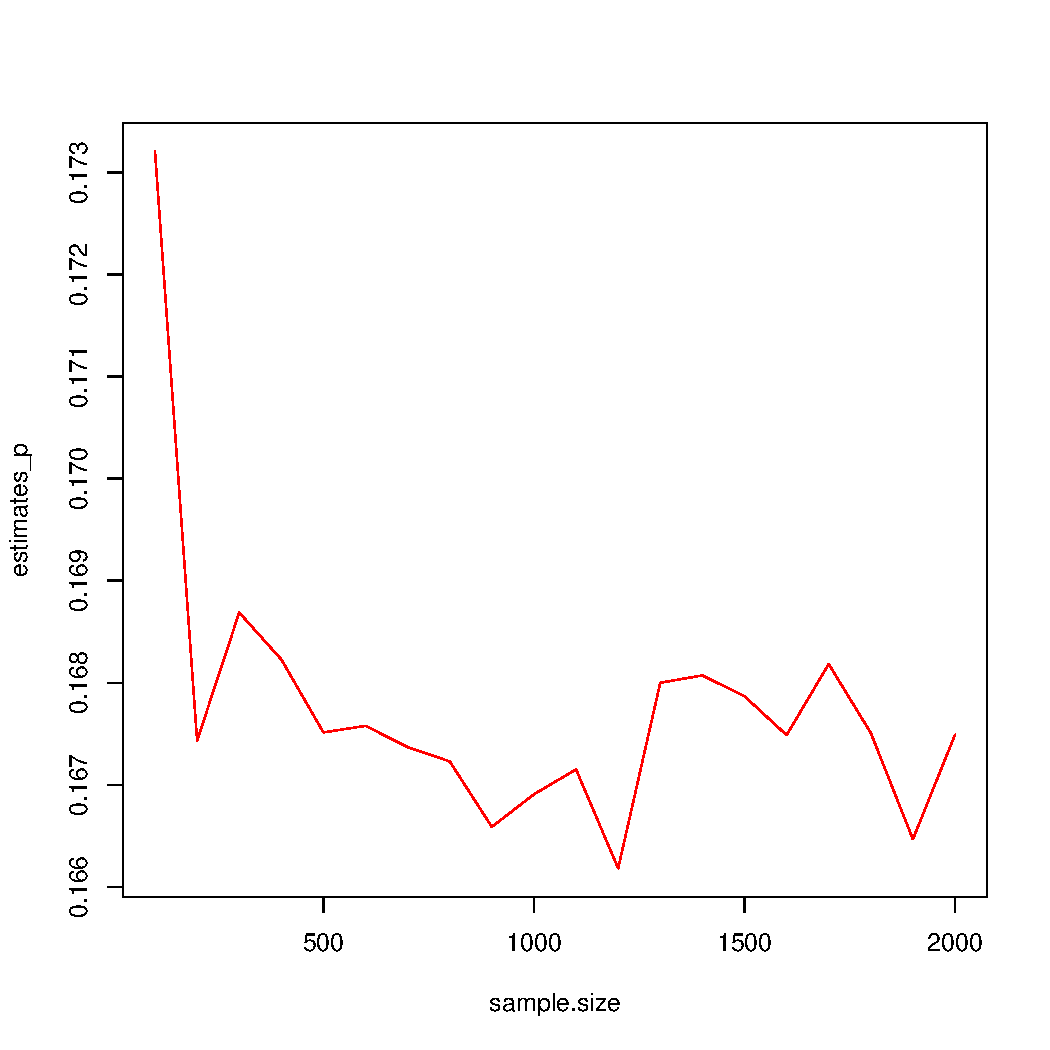
\includegraphics[width=\maxwidth]{figure/unnamed-chunk-9-1} 
\begin{kframe}\begin{alltt}
\hlkwd{plot}\hlstd{(sample.size, estimates_lmbd,} \hlkwc{type} \hlstd{=} \hlstr{"l"}\hlstd{,} \hlkwc{col} \hlstd{=} \hlstr{"red"}\hlstd{,} \hlkwc{ylim}\hlstd{=}\hlkwd{c}\hlstd{(}\hlnum{2.7}\hlstd{,} \hlnum{3.4}\hlstd{))}
\end{alltt}
\end{kframe}
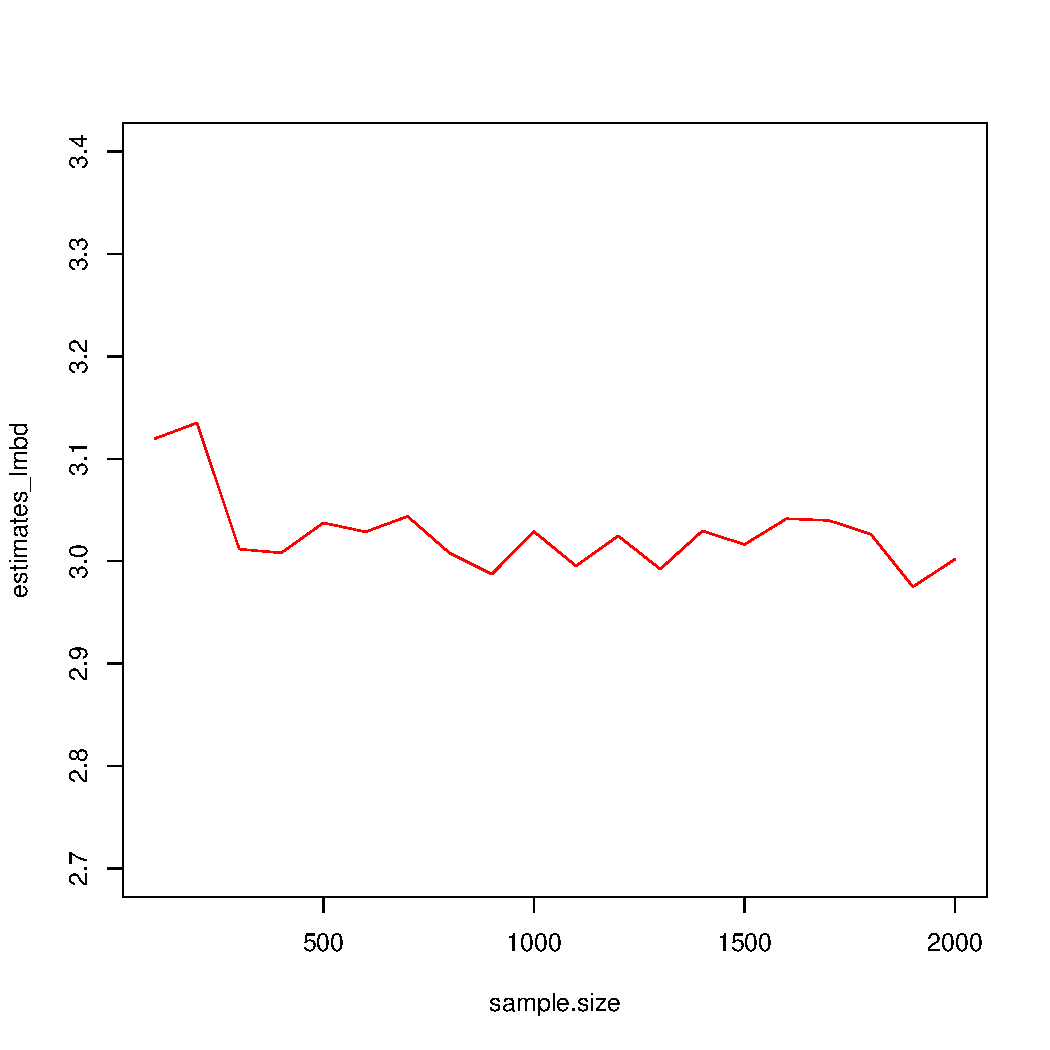
\includegraphics[width=\maxwidth]{figure/unnamed-chunk-9-2} 

\end{knitrout}

Мы видим, что оценка параметра $p$~--- смещенная, а следовательно не состоятельная.
Оценка параметра $\lambda$~--- несмещенная.

Теперь построим график дисперсии параметра $\lambda$, чтобы оценить состоятельность.

\begin{knitrout}
\definecolor{shadecolor}{rgb}{0.969, 0.969, 0.969}\color{fgcolor}\begin{kframe}
\begin{alltt}
\hlkwd{plot}\hlstd{(sample.size, estimates_lmbd_dh,} \hlkwc{type} \hlstd{=} \hlstr{"l"}\hlstd{,} \hlkwc{col} \hlstd{=} \hlstr{"red"}\hlstd{)}
\end{alltt}
\end{kframe}
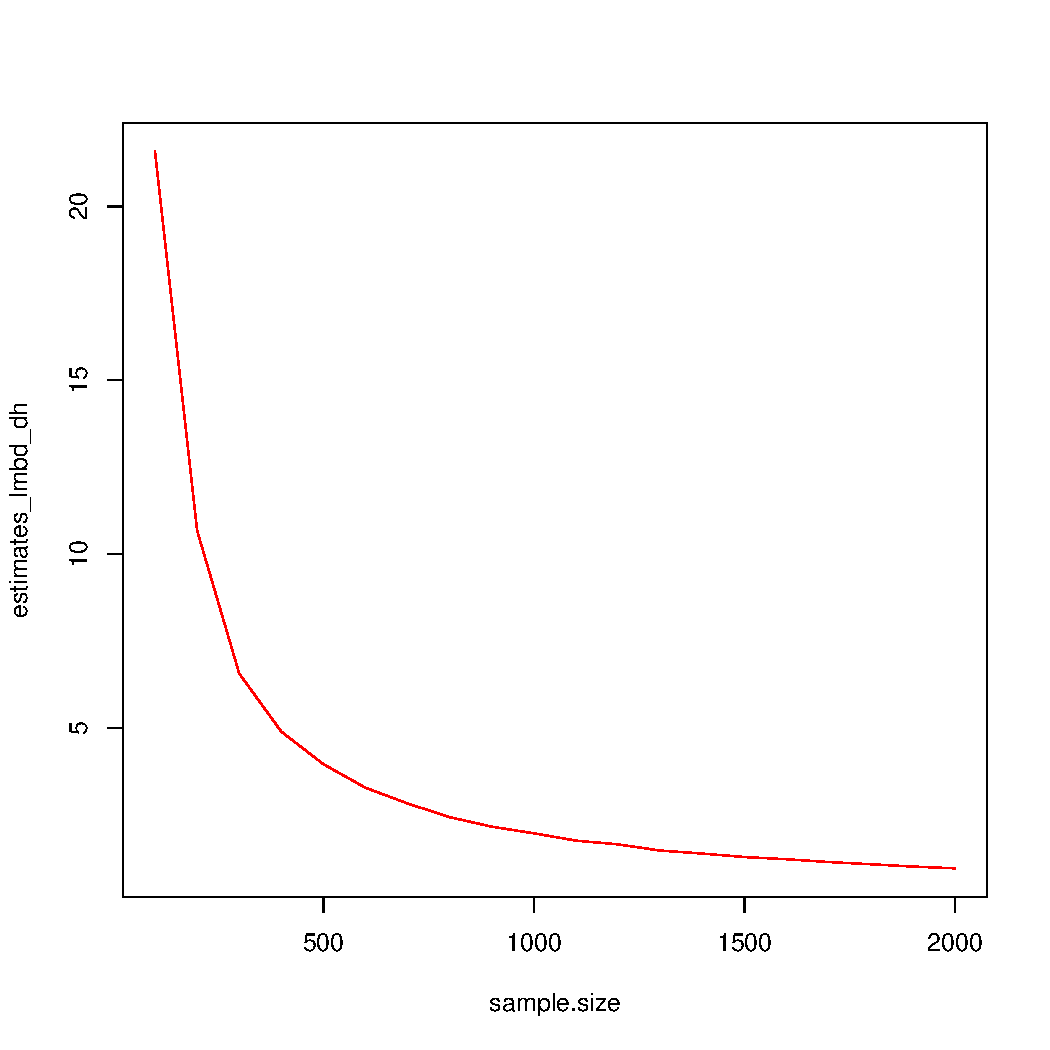
\includegraphics[width=\maxwidth]{figure/unnamed-chunk-10-1} 

\end{knitrout}

Дисперсия с ростом объема выборки стремиться к нулю из чего делаем вывод о состоятельности оценки $\lambda$.

Чтобы оценить достаточность оценок, рассмотрим функцию правдоподобия:

\[
L(k) = \prod_{s=1}^n \sum_{j=1}^{\infty} \frac{\lambda^j e^{-\lambda}}{j!} \frac{(j + k_s - 1)!}{(j - 1)! k_s!} p^j (1 - p)^k_s
\]

Невозможно свести функцию правдоподобия к виду, для параметров $\lambda$ и $p$:
\[
h(k)g(\bar \theta (k), \theta)
\]

Делаем вывод о том, что оценки не являются достаточными.

\newpage

\textbf{Метод правдоподобия.}

Сделаем оценку методом правдоподобия для первого варианта.

Возьмем гамма распределение gamma(k, r) с параметрами: $k = 3$, $r = 2$.

Функция правдоподобия имеет вид:

\[
L(x) = \frac{e^{n \bar x r^{-1}}}{r^{nk} \Gamma^n(k)} (\prod_{i = 1}^n x_i)^{k-1}
\]

Получаем уравнения:

\[
\frac{\partial \log(L)}{\partial k} = \log(r) + \psi(k) - \frac{1}{n} \sum_i \log(x_i) = 0
\]
\[
\frac{\partial \log(L)}{\partial r} =  \frac{n \bar x}{r^2} - \frac{nk}{r} = 0
\]

Тогда $r = \frac{\bar x}{k}$, а k выразим через уравнение: 
\[
\log(\bar x) - \log(k) + \psi(k) - \frac{1}{n} \sum_i \log(x_i) = 0
\]

\begin{knitrout}
\definecolor{shadecolor}{rgb}{0.969, 0.969, 0.969}\color{fgcolor}\begin{kframe}
\begin{alltt}
\hlstd{estimate_mmp} \hlkwb{<-} \hlkwa{function}\hlstd{(}\hlkwc{samp}\hlstd{)\{}
  \hlstd{C} \hlkwb{<-} \hlkwd{log}\hlstd{(}\hlkwd{mean}\hlstd{(samp))} \hlopt{-} \hlkwd{sum}\hlstd{(}\hlkwd{log}\hlstd{(samp))} \hlopt{/} \hlkwd{length}\hlstd{(samp)}

  \hlstd{Credibility_func} \hlkwb{<-} \hlkwa{function}\hlstd{(}\hlkwc{al}\hlstd{,} \hlkwc{const}\hlstd{)\{}
    \hlkwd{log}\hlstd{(al)} \hlopt{-} \hlkwd{digamma}\hlstd{(al)} \hlopt{+} \hlstd{const}
  \hlstd{\}}

  \hlstd{k} \hlkwb{<-} \hlkwd{uniroot}\hlstd{(Credibility_func,} \hlkwc{const} \hlstd{=} \hlopt{-}\hlstd{C,}
  \hlkwc{lower} \hlstd{=} \hlnum{10e-10}\hlstd{,} \hlkwc{upper} \hlstd{=} \hlnum{1000}\hlstd{,} \hlkwc{extendInt} \hlstd{=} \hlstr{"yes"}\hlstd{)}\hlopt{$}\hlstd{root}
  \hlstd{r} \hlkwb{<-} \hlkwd{mean}\hlstd{(samp)}\hlopt{/}\hlstd{k}
  \hlkwd{return}\hlstd{(}\hlkwd{c}\hlstd{(k, r))}
\hlstd{\}}

\hlstd{first} \hlkwb{<-} \hlkwd{rgamma}\hlstd{(}\hlnum{100}\hlstd{,} \hlkwc{shape} \hlstd{=} \hlnum{3}\hlstd{,} \hlkwc{scale} \hlstd{=} \hlnum{2}\hlstd{)}
\hlstd{second} \hlkwb{<-} \hlkwd{rgamma}\hlstd{(}\hlnum{300}\hlstd{,} \hlkwc{shape} \hlstd{=} \hlnum{3}\hlstd{,} \hlkwc{scale} \hlstd{=} \hlnum{2}\hlstd{)}
\end{alltt}
\end{kframe}
\end{knitrout}
Оценки параметров для первой выборки:

\begin{knitrout}
\definecolor{shadecolor}{rgb}{0.969, 0.969, 0.969}\color{fgcolor}\begin{kframe}
\begin{alltt}
\hlstd{k_f} \hlkwb{<-} \hlkwd{estimate_mmp}\hlstd{(first)[}\hlnum{1}\hlstd{]}
\hlstd{r_f} \hlkwb{<-} \hlkwd{estimate_mmp}\hlstd{(first)[}\hlnum{2}\hlstd{]}
\hlkwd{c}\hlstd{(k_f, r_f)}
\end{alltt}
\begin{verbatim}
## [1] 3.484572 1.811735
\end{verbatim}
\end{kframe}
\end{knitrout}
Оценки параметров для второй выборки:

\begin{knitrout}
\definecolor{shadecolor}{rgb}{0.969, 0.969, 0.969}\color{fgcolor}\begin{kframe}
\begin{alltt}
\hlstd{k_s} \hlkwb{<-} \hlkwd{estimate_mmp}\hlstd{(second)[}\hlnum{1}\hlstd{]}
\hlstd{r_s} \hlkwb{<-} \hlkwd{estimate_mmp}\hlstd{(second)[}\hlnum{2}\hlstd{]}
\hlkwd{c}\hlstd{(k_s, r_s)}
\end{alltt}
\begin{verbatim}
## [1] 3.396228 1.737584
\end{verbatim}
\end{kframe}
\end{knitrout}
Построим доверительный интервал для оценок:

\begin{knitrout}
\definecolor{shadecolor}{rgb}{0.969, 0.969, 0.969}\color{fgcolor}\begin{kframe}
\begin{alltt}
\hlstd{D_k} \hlkwb{<-} \hlnum{1} \hlopt{/} \hlstd{(}\hlkwd{length}\hlstd{(first)} \hlopt{*} \hlstd{(}\hlkwd{psigamma}\hlstd{(k_f)} \hlopt{-} \hlnum{1} \hlopt{/} \hlstd{k_f))}
\hlstd{D_r} \hlkwb{<-} \hlstd{r_f}\hlopt{^}\hlnum{2} \hlopt{/} \hlstd{(}\hlkwd{length}\hlstd{(first)} \hlopt{*} \hlstd{(k_f} \hlopt{-} \hlnum{1} \hlopt{/} \hlkwd{psigamma}\hlstd{(}\hlnum{10}\hlstd{)))}

\hlstd{D_k2} \hlkwb{<-} \hlnum{1} \hlopt{/} \hlstd{(}\hlkwd{length}\hlstd{(second)} \hlopt{*} \hlstd{(}\hlkwd{psigamma}\hlstd{(k_s)} \hlopt{-} \hlnum{1} \hlopt{/} \hlstd{k_s))}
\hlstd{D_r2} \hlkwb{<-} \hlstd{r_s}\hlopt{^}\hlnum{2} \hlopt{/} \hlstd{(}\hlkwd{length}\hlstd{(second)} \hlopt{*} \hlstd{(k_s} \hlopt{-} \hlnum{1} \hlopt{/} \hlkwd{psigamma}\hlstd{(k_s)))}
\end{alltt}
\end{kframe}
\end{knitrout}
Для параметра $k$, 95\% доверительный интервал первой и второй выборки соответственно:

\begin{knitrout}
\definecolor{shadecolor}{rgb}{0.969, 0.969, 0.969}\color{fgcolor}\begin{kframe}
\begin{alltt}
\hlkwd{c}\hlstd{(k_f} \hlopt{-} \hlkwd{qnorm}\hlstd{(}\hlnum{0.975}\hlstd{)}\hlopt{*}\hlkwd{sqrt}\hlstd{(D_k} \hlopt{/} \hlstd{n1), k_f} \hlopt{+} \hlkwd{qnorm}\hlstd{(}\hlnum{0.975}\hlstd{)}\hlopt{*}\hlkwd{sqrt}\hlstd{(D_k} \hlopt{/} \hlstd{n1))}
\end{alltt}
\begin{verbatim}
## [1] 3.462809 3.506335
\end{verbatim}
\begin{alltt}
\hlkwd{c}\hlstd{(k_s} \hlopt{-} \hlkwd{qnorm}\hlstd{(}\hlnum{0.975}\hlstd{)}\hlopt{*}\hlkwd{sqrt}\hlstd{(D_k2} \hlopt{/} \hlstd{n2), k_s} \hlopt{+} \hlkwd{qnorm}\hlstd{(}\hlnum{0.975}\hlstd{)}\hlopt{*}\hlkwd{sqrt}\hlstd{(D_k2} \hlopt{/} \hlstd{n2))}
\end{alltt}
\begin{verbatim}
## [1] 3.388801 3.403655
\end{verbatim}
\end{kframe}
\end{knitrout}

Для параметра $r$, 95\% доверительный интервал первой и второй выборки соответственно:

\begin{knitrout}
\definecolor{shadecolor}{rgb}{0.969, 0.969, 0.969}\color{fgcolor}\begin{kframe}
\begin{alltt}
\hlkwd{c}\hlstd{(r_f} \hlopt{-} \hlkwd{qnorm}\hlstd{(}\hlnum{0.975}\hlstd{)}\hlopt{*}\hlkwd{sqrt}\hlstd{(D_r} \hlopt{/} \hlstd{n1), r_f} \hlopt{+} \hlkwd{qnorm}\hlstd{(}\hlnum{0.975}\hlstd{)}\hlopt{*}\hlkwd{sqrt}\hlstd{(D_r} \hlopt{/} \hlstd{n1))}
\end{alltt}
\begin{verbatim}
## [1] 1.791370 1.832099
\end{verbatim}
\begin{alltt}
\hlkwd{c}\hlstd{(r_s} \hlopt{-} \hlkwd{qnorm}\hlstd{(}\hlnum{0.975}\hlstd{)}\hlopt{*}\hlkwd{sqrt}\hlstd{(D_r2} \hlopt{/} \hlstd{n2), r_s} \hlopt{+} \hlkwd{qnorm}\hlstd{(}\hlnum{0.975}\hlstd{)}\hlopt{*}\hlkwd{sqrt}\hlstd{(D_r2} \hlopt{/} \hlstd{n2))}
\end{alltt}
\begin{verbatim}
## [1] 1.730346 1.744822
\end{verbatim}
\end{kframe}
\end{knitrout}

оценим несмещенность оценок:

\begin{knitrout}
\definecolor{shadecolor}{rgb}{0.969, 0.969, 0.969}\color{fgcolor}\begin{kframe}
\begin{alltt}
\hlstd{sample.size} \hlkwb{<-} \hlkwd{seq}\hlstd{(}\hlnum{100}\hlstd{,} \hlnum{5000}\hlstd{,} \hlkwc{by} \hlstd{=} \hlnum{100}\hlstd{)}

\hlstd{estimates_r} \hlkwb{<-} \hlkwd{character}\hlstd{()}
\hlstd{estimates_k} \hlkwb{<-} \hlkwd{character}\hlstd{()}

\hlkwa{for} \hlstd{(size} \hlkwa{in} \hlstd{sample.size) \{}
  \hlstd{temp_r} \hlkwb{<-} \hlkwd{character}\hlstd{()}
  \hlstd{temp_k} \hlkwb{<-} \hlkwd{character}\hlstd{()}
  \hlkwa{for} \hlstd{(i} \hlkwa{in} \hlnum{1}\hlopt{:}\hlnum{100}\hlstd{) \{}
    \hlstd{temp} \hlkwb{<-} \hlkwd{rgamma}\hlstd{(size,} \hlkwc{shape} \hlstd{=} \hlnum{3}\hlstd{,} \hlkwc{scale} \hlstd{=} \hlnum{2}\hlstd{)}
    \hlstd{y} \hlkwb{<-} \hlkwd{estimate_mmp}\hlstd{(temp)}
    \hlstd{temp_k} \hlkwb{<-} \hlkwd{c}\hlstd{(temp_k, y[}\hlnum{1}\hlstd{])}
    \hlstd{temp_r} \hlkwb{<-} \hlkwd{c}\hlstd{(temp_r, y[}\hlnum{2}\hlstd{])}
  \hlstd{\}}

  \hlstd{temp_k} \hlkwb{<-} \hlkwd{as.numeric}\hlstd{(temp_k)}
  \hlstd{temp_r} \hlkwb{<-} \hlkwd{as.numeric}\hlstd{(temp_r)}

  \hlstd{estimates_r} \hlkwb{<-} \hlkwd{c}\hlstd{(estimates_r,} \hlkwd{mean}\hlstd{(temp_r))}
  \hlstd{estimates_k} \hlkwb{<-} \hlkwd{c}\hlstd{(estimates_k,} \hlkwd{mean}\hlstd{(temp_k))}
\hlstd{\}}

\hlstd{estimates_k} \hlkwb{<-} \hlkwd{as.numeric}\hlstd{(estimates_k)}
\hlstd{estimates_r} \hlkwb{<-} \hlkwd{as.numeric}\hlstd{(estimates_r)}

\hlkwd{plot}\hlstd{(sample.size, estimates_r,} \hlkwc{type} \hlstd{=} \hlstr{"l"}\hlstd{,} \hlkwc{col} \hlstd{=} \hlstr{"red"}\hlstd{,} \hlkwc{ylim}\hlstd{=}\hlkwd{c}\hlstd{(}\hlnum{1.8}\hlstd{,} \hlnum{2.2}\hlstd{))}
\end{alltt}
\end{kframe}
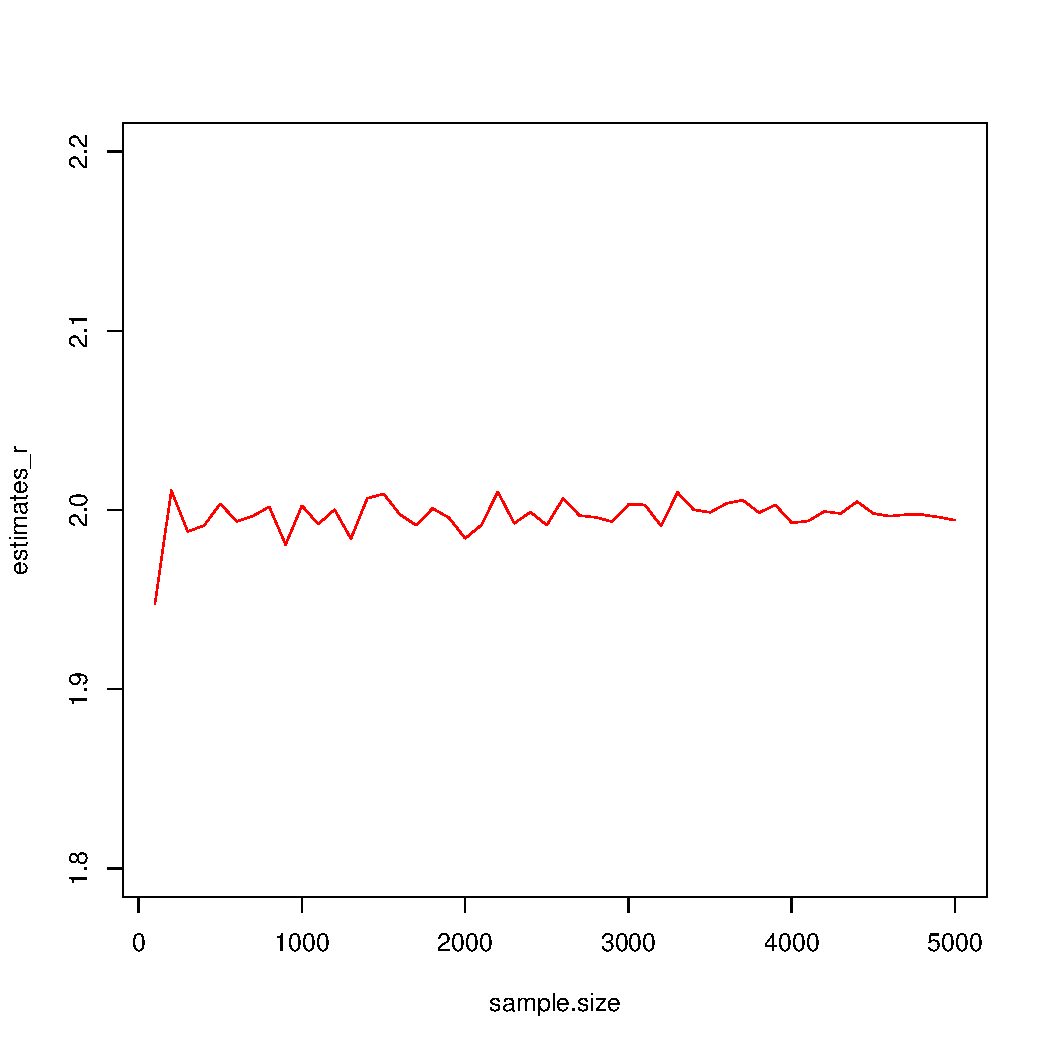
\includegraphics[width=\maxwidth]{figure/unnamed-chunk-17-1} 
\begin{kframe}\begin{alltt}
\hlkwd{plot}\hlstd{(sample.size, estimates_k,} \hlkwc{type} \hlstd{=} \hlstr{"l"}\hlstd{,} \hlkwc{col} \hlstd{=} \hlstr{"red"}\hlstd{,} \hlkwc{ylim}\hlstd{=}\hlkwd{c}\hlstd{(}\hlnum{2.8}\hlstd{,} \hlnum{3.2}\hlstd{))}
\end{alltt}
\end{kframe}
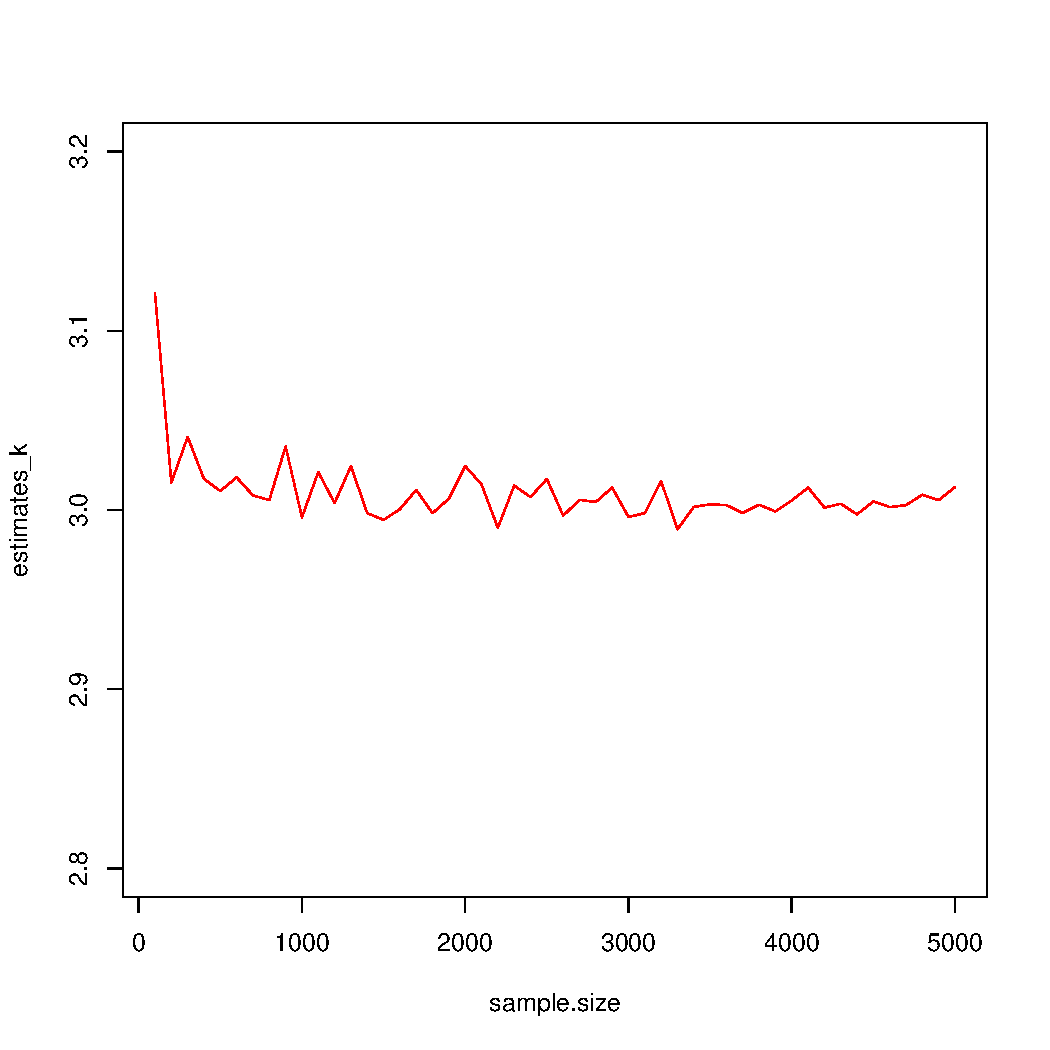
\includegraphics[width=\maxwidth]{figure/unnamed-chunk-17-2} 

\end{knitrout}

Для обеих оценок из графика устанавливаем, что при увеличении объема выборки, среднее сходится к истинному значению, делаем вывод, что оценки несмещенные.

Для оценок ММП известно, что они являются состоятельными и ассимптотически эффективными.

\end{document}
